\documentclass[letterpaper,10pt]{article}
\usepackage{graphicx}
\usepackage{listings}
\usepackage{fullpage}
\usepackage{fixltx2e}
\usepackage{multirow}
\usepackage{amssymb,amsmath}
\usepackage{mathtools}
\usepackage{bm}
\usepackage[hyperfootnotes=false]{hyperref}
\usepackage{url}
\usepackage{subfig}
\usepackage{relsize}
\usepackage{enumitem}
\usepackage{fancyhdr}
\usepackage{framed}
\setlength{\headheight}{14pt}
\pagestyle{fancy}
\headsep = 20pt

% Lineskip mods
\linespread{1.0}
\setlength{\parskip}{0.5\baselineskip}
\setlength{\parindent}{0pt}
\newlength\docparskip
\parskip=6pt
\setlength{\docparskip}{\parskip}
\renewcommand{\arraystretch}{1.085}
\usepackage{xcolor}
\lstset{basicstyle=\ttfamily,
  showstringspaces=false,
  commentstyle=\color{red},
  keywordstyle=\color{blue}
}
\begin{document}

\fancyhf{}
\fancyhead[L]{AME 60614: Numerical Methods}
\fancyhead[R]{Qihao Zhuo: Problem Set 0}
\fancyfoot[C]{\thepage}

\thispagestyle{plain}
\begin{center}
  \large
  \textbf{AME 60614: Numerical Methods} \\
  \textbf{Fall 2021} \\
  \vspace{0.5em}
  \textbf{Problem Set 1} \\
  \vspace{1em}
  Qihao Zhuo
\end{center}

\vspace{1.5em}

All revised codes are included in tar file. There are statements describing which parts were revised 
at the beginning of each problem. 

\section{Finite-Difference Schemes}\label{sec1}
In my former homework, I got full points in Problem 1 so I did not revise this problem. 
\subsection{$f_{i-2},f_{i-1},f_{i},f_{i+1},f_{i+2}$}
With the MATLAB scripts $p1\_1.m$, coefficients solved by corresponding matrix equation are shown in the Tab.~\ref{tab1_1}.  
\begin{table}[htbp]
  \centering  
  \caption{Output of First Group}\label{tab1_1}
  \begin{tabular}{cccccccc}
    \hline
    & $a_1$ & $a_2$ & $a_3$ & $a_4$& $a_5$ & $Truncation Error$& $Accuracy$\\
    \hline
    $f_{i}^{''}$ & $\frac{-1}{12h^2}$ & $\frac{4}{3h^2}$ & $\frac{-5}{2h^2}$ & $\frac{4}{3h^2}$ & $\frac{-1}{12h^2}$ & $\frac{h^4}{90}f_{i}^{6}$& $O\left(h^4\right)$\\
    $f_{i}^{iv}$ & $\frac{1}{h^4}$ & $\frac{-4}{h^4}$ & $\frac{6}{h^4}$ & $\frac{-4}{h^4}$ & $\frac{1}{h^4}$ & $\frac{-h^2}{6}f_{i}^{6}$& $O\left(h^2\right)$\\
    $f_{i}^{'''}-3f_{i}^{'}$ & $\frac{-\left(h^2+2\right)}{4h^3}$ & $\frac{2h^2+1}{h^3}$ & 0 & $\frac{-\left(h^2+1\right)}{h^3}$ & $\frac{h^2+2}{4h^3}$ & $\left(\frac{2h^2(h^2 + 2)}{15} - \frac{h^2(2h^2 + 1)}{60}\right)f_{i}^{5}$&$O\left(h^2\right)$\\
    \hline
  \end{tabular}
\end{table}
\subsection{$f_{i},f_{i+1},f_{i+2},f_{i+3},f_{i+4}$}
With the MATLAB scripts $p1\_2.m$, coefficients are shown in the Tab.~\ref{tab1_2}.  
\begin{table}[htbp]
  \centering  
  \caption{Output of Second Group}\label{tab1_2}
  \begin{tabular}{cccccccc}
    \hline
    & $a_1$ & $a_2$ & $a_3$ & $a_4$& $a_5$ & Truncation Error& Accuracy\\
    \hline
    $f_{i}^{''}$ & $\frac{35}{12h^2}$ & $\frac{-26}{3h^2}$ & $\frac{19}{2h^2}$ & $\frac{-14}{3h^2}$ & $\frac{11}{12h^2}$ & $-\frac{5h^3}{6}f_{i}^{5}$& $O\left(h^3\right)$\\
    $f_{i}^{iv}$ & $\frac{1}{h^4}$ & $\frac{-4}{h^4}$ & $\frac{6}{h^4}$ & $\frac{-4}{h^4}$ & $\frac{1}{h^4}$ & $-2hf_{i}^{5}$& $O\left(h\right)$\\
    $f_{i}^{'''}-3f_{i}^{'}$ & $\frac{5\left(5h^2-2\right)}{4h^3}$ & $\frac{-3\left(4h^2-3\right)}{h^3}$ & $\frac{3\left(3h^2-4\right)}{h^3}$ & $\frac{-\left(4h^2-7\right)}{h^3}$ & $\frac{3\left(h^2-2\right)}{4h^3}$ & Eq.~\ref{p1eq1}&$O\left(h^2\right)$\\
    \hline
  \end{tabular}
\end{table}
\begin{equation}\label{p1eq1}
  TE = -\left(\frac{32h^2(h^2 - 2)}{5} + \frac{4h^2(3h^2 - 4)}{5} - \frac{h^2(4h^2 - 3)}{40} - \frac{81h^2(4h^2 - 7)}{40}\right)f_{i}^{5}
\end{equation}
\subsection{$f_{i-4},f_{i-3},f_{i-2},f_{i-1},f_{i}$}
With the MATLAB scripts $p1\_3.m$, coefficients are shown in the Tab.~\ref{tab1_3}
\begin{table}[htbp]
  \centering  
  \caption{Output of Third Group}\label{tab1_3}
  \begin{tabular}{cccccccc}
    \hline
    & $a_1$ & $a_2$ & $a_3$ & $a_4$& $a_5$ & Truncation Error& Accuracy\\
    \hline
    $f_{i}^{''}$ & $\frac{11}{12h^2}$ & $\frac{-14}{3h^2}$ & $\frac{19}{2h^2}$ & $\frac{-26}{3h^2}$ & $\frac{35}{12h^2}$ & $\frac{5h^3}{6}f_{i}^{5}$& $O\left(h^3\right)$\\
    $f_{i}^{iv}$ & $\frac{1}{h^4}$ & $\frac{-4}{h^4}$ & $\frac{6}{h^4}$ & $\frac{-4}{h^4}$ & $\frac{1}{h^4}$ & $2hf_{i}^{5}$& $O\left(h\right)$\\
    $f_{i}^{'''}-3f_{i}^{'}$ & $\frac{-3\left(h^2-2\right)}{4h^3}$ & $\frac{4h^2-7}{h^3}$ & $\frac{-3\left(3h^2-4\right)}{h^3}$ & $\frac{3\left(4h^2-3\right)}{h^3}$ & $\frac{-5\left(5h^2-2\right)}{4h^3}$ & Eq.~\ref{p1eq2}&$O\left(h^2\right)$\\
    \hline
  \end{tabular}
\end{table}
\begin{equation}\label{p1eq2}
  TE = -\left(\frac{32h^2(h^2 - 2)}{5} + \frac{4h^2(3h^2 - 4)}{5} - \frac{h^2(4h^2 - 3)}{40} - \frac{81h^2(4h^2 - 7)}{40}\right)f_{i}^{5}
\end{equation}
\subsection{$f_{i-1},f_{i},f_{i+1},f_{i-1}^{'},f_{i}^{'},f_{i+1}^{'}$}
With the MATLAB scripts $p1\_4.m$, coefficients are shown in the Tab.~\ref{tab1_4}. 
\begin{table}[htbp]
  \centering  
  \caption{Output of Fourth Group}\label{tab1_4}
  \begin{tabular}{ccccccccc}
    \hline
    & $a_1$ & $a_2$ & $a_3$ & $a_4$& $a_5$ & $a_6$& Truncation Error& Accuracy\\
    \hline
    $f_{i}^{''}$ & $\frac{2}{h^2}$ & $\frac{-4}{h^2}$ & $\frac{2}{2h^2}$ & $\frac{1}{2h}$ &0& $\frac{-1}{2h}$ & $\frac{h^4}{360}f_{i}^{6}$& $O\left(h^4\right)$\\
    $f_{i}^{iv}$ & $\frac{-12}{h^4}$ & $\frac{24}{h^4}$ & $\frac{-12}{h^4}$ & $\frac{-6}{h^3}$ &0& $\frac{6}{h^3}$ & $-\frac{h^2}{15}f_{i}^{6}$& $O\left(h^2\right)$\\
    $f_{i}^{'''}-3f_{i}^{'}$ & $\frac{15}{2h^3}$ & $0$ & $\frac{15}{2h^3}$ & $\frac{-3}{2h^2}$ & $\frac{-3\left(h^2+4\right)}{h^2}$ & $\frac{-3}{2h^2}$&$\frac{h^4}{840}f_{i}^{7}$&$O\left(h^4\right)$\\
    \hline
  \end{tabular}
\end{table}

\section{Richardson Extrapolation}
I used explicit formula for even 10-order scheme, which will made too small fractions. 
So I revised this problem with solution' s idea. To use vector easily, I wrote a new matlab code 
$p2\_2\_{rev}.m$ to solve this problem. 

\subsection{a}
For fourth-order central-difference scheme, fivr points are required. Modifying codes in Sec. \ref{sec1} to solve named 
the scheme with points of $x-2h, x-h, x, x+h, x+2h$. 
\begin{align*}
  \frac{1}{12h}f_{i-2}-\frac{2}{3}f_{i-1}+\frac{2}{3}f_{i+1}-\frac{1}{12}f_{i+2}
  &= f_{i}^{'} - \frac{h^4}{30} - \frac{h^6}{252} - \frac{h^8}{4320} - \frac{17h^{10}}{1995840}\\
  D_i&=f_{i}^{'}
\end{align*}

Under central-difference scheme, the odd-order terms are zero. So to get sixth-, eighth- and tenth- order
schemes, solving corresponding linear equations need two, three and four expressions.

\begin{align*}
  D_1&=D-c_1h^4-c_2h^6-c_3h^8-c_4h^10+...\\
  D_{12}&=\frac{16D_2-D_1}{15}=D+c_2\frac{h^6}{20}+c_3\frac{h^8}{16}+c_4\frac{21h^{10}}{320}+...\\
  D_{123} &=\frac{64D_{23}-D_{12}}{63}=D-c_3\frac{h^8}{1344}-c_4\frac{h^{10}}{1024}+...\\
  D^{1234} &=\frac{256D_{234}-D_{123}}{255}=D+c_4\frac{h^{10}}{208896}+...
\end{align*}
\subsection{b}
With $p2\_2\_{rev}.m$, output of different schemes under $x=1$ and $h=0.5,0.25,0.1,0.05,0.025$ is shown in Fig.~\ref{fig2_1}. 

\begin{figure}[h]
  \centering
  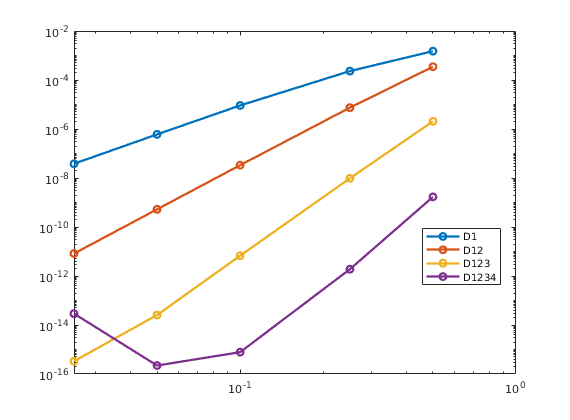
\includegraphics[width=0.5\textwidth]{p2_1.png}
  \caption{$\log |\epsilon|-\log h$ of different $h$ and different schemes}
  \label{fig2_1}
\end{figure}

\begin{align*}
  |\epsilon|&\propto h^2\\
  \log |\epsilon| \propto \log h^2&= 2\log h
\end{align*}

The slopes of different lines of $D_1,D_{12},D_{123},D_{1234}$ are about $4,6,8,10$ correspondingly, 
which implies those schemes have the correct accuracy. 
\section{Integral Equations}
In this problem, I just modied my code to output errors of different $x_i$ and $N$. 
The algorithm is almost correct. 
\subsection{a}
With the trapezoid method, the integral term could be approximated, 
\begin{equation}
  \int_0^x K\left(x,t\right)f\left(t\right)\mathrm{d}t \approx \frac{\Delta t}{2}
  \left[K\left(x,t_0\right)f\left(t_0\right)+2K\left(x,t_1\right)f\left(t_1\right)+...+2K\left(x,t_{n-1}\right)f\left(t_{n-1}+K\left(x,t_n\right)f\left(t_n\right)\right)\right]\notag
\end{equation}

Taking $f\left(t_i\right)=f_i$, $g\left(x_i\right) = g_i$ and $K_{ij} = K\left(x_i,t_j\right)$. 
\begin{align}
    f_0 &= g_0\notag\\
    f_1 + \frac{\Delta t}{2}\left(K_{10}f_0 + K_{11}f_1\right) &= g_1\notag\\
    f_2 + \frac{\Delta t}{2}\left(K_{20}f_0 + 2K_{21}f_1 + K_{22}f_2\right) &= g_2\notag\\
    &...\notag\\
    f_n + \frac{\Delta t}{2}\left(K_{n0}f_0 + 2K_{n1}f_1 + ...+ 2K_{n,n-1}f_{n-1}+K_{n,n}f_n\right) &= g_n\notag
\end{align}

Adding $f_i$ term into the trapezoid term, 
\begin{align}
  f_0 &= g_0\notag\\
  \frac{\Delta t}{2}\left[K_{10}f_0 + \left(K_{11}+1\right)f_1\right] &= g_1\notag\\
  \frac{\Delta t}{2}\left[K_{20}f_0 + 2K_{21}f_1 + \left(K_{22}+1\right)f_2\right] &= g_2\notag\\
  &...\notag\\
  \frac{\Delta t}{2}\left[K_{n0}f_0 + 2K_{n1}f_1 + ...+ 2K_{n,n-1}f_{n-1}+\left(K_{n,n}+1\right)f_n\right] &= g_n\notag
\end{align}

Those equations could be seen as a linear equations system. 
\begin{align}
  \bm{Mf} &= \bm{g}\notag\\
  \bm{f} &= \bm{M}^{-1}\bm{g}\notag
\end{align}

Through solving such matrix equation, a discret set of approximate values of $f\left(x\right)$ will be given. 
The trapezoid method has a accuracy of $O\left(h^2\right)$. From the matrix equation, accuracy of $f\left(x\right)$ also has the accuracy of $O\left(h^2\right)$. 
\subsection{b}
The analytical solution is unknown, so pseudo-error is used. An approximation under 
grid spacing $h$ can be written as:
\begin{equation*}
  f^*_h=f_e+c_1h^n
\end{equation*}

Where $f_e$ is the exact value. For grid spacing $h/2$, the approimation is, 
\begin{equation*}
  f^*_{h/2}=f_e+c_1\left(\frac{h}{2}\right)^n
\end{equation*}

So the pseudo-error could be derived. 
\begin{equation*}
  \epsilon = f^*_h-f^*_{h/2}=c_1\left(1-2^{-n}\right)h^n=c_2h^n
\end{equation*}

In that probelm, the algorithm has accuracy of $O\left(h^2\right)$. 
\begin{align*}
  |\epsilon|&\propto h^2\\
  \log |\epsilon| \propto \log h^2= 2\log h &= 2\log \frac{L}{N}\\
  \log |\epsilon| &\propto -2 \log N
\end{align*}

Therefore the $\log \epsilon-\log N$ plots should be linear and the slope should be $-2$. 

Using $p3\_1_{rev}.m$, the algorithm defined above is written as a function. Different cases are 
simulated under $N=10,100,500,1000,5000,10000$ and $x_i=0.2,0.5,1.0$, and $\log \epsilon-\log N$ plots are shown in Fig.~\ref{fig3_2}. 
The $f(x)$ under $N=10000$ is shown in Fig.~\ref{fig3_1}. 

\begin{figure}[h]
  \centering
  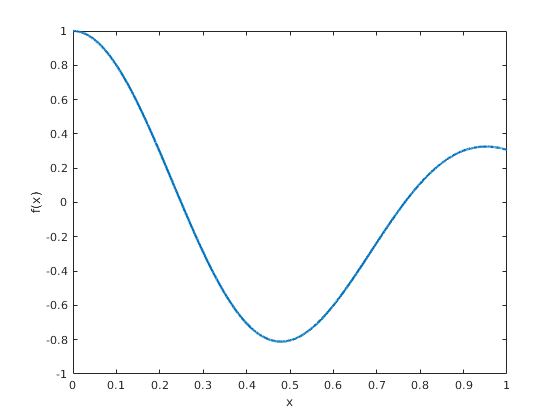
\includegraphics[width=0.5\textwidth]{p3_1.png}
  \caption{Figure of $f(x)$ under $N=10000$}
  \label{fig3_1}
\end{figure}

\begin{figure}[h]
  \centering
  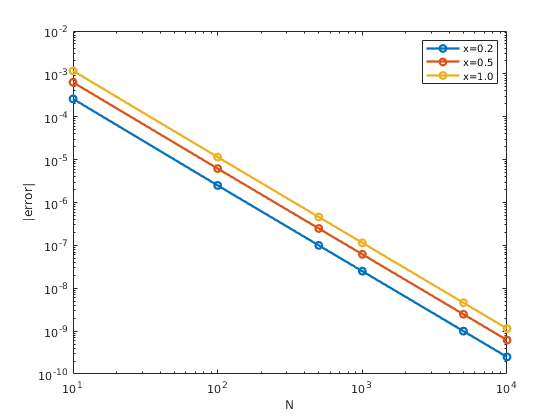
\includegraphics[width=0.5\textwidth]{p3_2.png}
  \caption{$\log |\epsilon|-\log N$ under $N=10,100,500,1000,5000,100000$ and $x=0.2,0.5,1.0$}
  \label{fig3_2}
\end{figure}

The $\log \epsilon-\log N$ plots are linear and the slope is nearly $-2$, so the algorithm in this problem has 
accuracy of $O\left(h^2\right)$. 
\section{Gauss-Hermite Quadrature}
In my former work, the Gauss-Hermite Quadrature part is totally correct. So I just revised this problem 
on the Simpson part with solution' s idea. I also refer to points setting in the solution, but my results 
are good enough. 
\subsection{a}
The original integral interval is $\left(-\infty,\infty\right)$, which cannot be achieved by simulations. 
So a transform should be used. 
\begin{align*}
  \xi&=\tanh x\\
  x&=\tanh ^{-1} \xi\\
  dx&=\frac{1}{1-\xi ^2}d\xi
\end{align*}

So that the integral interval becomes $\left[-1,1\right]$. 
\begin{align*}
  I&=\int^1_{-1}F\left(\xi\right)d\xi=\int^1_{-1}f\left(\tanh^{-1}\xi\right)\left[\frac{1}{\sqrt{2\pi}}e^{-\left(\tanh^{-1}\xi\right)^2/2}\right]\frac{1}{1-\xi ^2}d\xi\\
  I_{Simpson}&=\frac{h}{3}\left(F_0+F_{n}+4\sum^{n-1}_{j=1,odd}F_j+2\sum^{n-2}_{j=2,even}F_j\right)
\end{align*}

With code of Simpson's rule, $p4\_1\_{rev}.f90$, the three numerical integrals are shown in Tab.~\ref{tab4_1}. 
From Tab.~\ref{tab4_1}, the points required to achieve the error of $\epsilon=10^{-6}$ for each case are also shown. 
\begin{table}[htbp]
  \centering  
  \caption{Simpson method for different moments}\label{tab4_1}
  \begin{tabular}{cccccc}
    \hline
    & $I_{Simpson}$ & $I_{exact}$ & $Absolute Error$ & $Relative Error$& $n$\\
    \hline
    1 & 1.0000009915918198 & 1 & 9.9159181976560262E-007 & 9.9159181976560262E-007 & 5900\\
    $x^2$ & 1.0000009526069624 & 1 & 9.5260696242327469E-007 & 9.5260696242327469E-007 & 24000\\
    $x^4$ & 3.0000009925061115 & 3 & 9.9250611151902035E-007 & 3.3083537050634010E-007 & 90000\\
    \hline
  \end{tabular}
\end{table}
\subsection{b}
The general form of Gauss-Hermite Quadrature is using $e^{-x^2}$, so a variable changing of $x=\sqrt{2}t$ 
is used to modify the function form. 
\begin{align}
  \int_{-\infty}^{\infty} \left[\frac{1}{\sqrt{2\pi}}e^{\frac{-x^2}{2}}\right]\mathrm{d}x &= \frac{1}{\sqrt{\pi}}\int_{-\infty}^{\infty} e^{-t^2}\mathrm{d}t\notag\\
  \int_{-\infty}^{\infty} x^2\left[\frac{1}{\sqrt{2\pi}}e^{\frac{-x^2}{2}}\right]\mathrm{d}x &= \frac{1}{\sqrt{\pi}}\int_{-\infty}^{\infty} 2t^2 e^{-t^2}\mathrm{d}t\notag\\
  \int_{-\infty}^{\infty} x^4\left[\frac{1}{\sqrt{2\pi}}e^{\frac{-x^2}{2}}\right]\mathrm{d}x &= \frac{1}{\sqrt{\pi}}\int_{-\infty}^{\infty} 4t^4 e^{-t^2}\mathrm{d}t\notag\\
  \int_{-\infty}^{\infty} \cos x \left[\frac{1}{\sqrt{2\pi}}e^{\frac{-x^2}{2}}\right]\mathrm{d}x &= \frac{1}{\sqrt{\pi}}\int_{-\infty}^{\infty} \cos \left(\sqrt{2}t\right) e^{-t^2}\mathrm{d}t\notag
\end{align}

For $f\left(x\right)=x^2$, $2N+1=2 \Rightarrow N+1=1.5$. So 2 points would be required to exactly compute it. 

For $f\left(x\right)=x^4$, $2N+1=4 \Rightarrow N+1=2.5$. So 3 points would be required to exactly compute it. 

The output of Gauss-Hermite Quadrature of second moments with 2 points and fourth moments with 4 points is shown in Tab.~\ref{tab4_2}. 
The conclusion is \underline{verified}. 
\begin{table}[htbp]
  \centering  
  \caption{Gauss-Hermite Quadrature for different moments}\label{tab4_2}
  \begin{tabular}{ccccc}
    \hline
    & $I_{G-H}$ & $I_{exact}$ & $Absolute Error$ & $Quadrature Points$\\
    \hline
    $x^2$ & 1 & 1 & 0 & 2\\
    $x^4$ & 3 & 3 & 0 & 3\\
    \hline
  \end{tabular}
\end{table}

\subsection{c}
Modifying $p4\_2.mlx$ and $p4\_1\_{rev}.f90$, output is shown in Tab.~\ref{tab4_3} and points required to 
achive the error of $\epsilon=10^{-6}$ for each case are also shown. For Simpson, 5200 points are required. 
For Gauss-Heremite Quadrature, $N=6$ leads to an error more than $10^{-6}$ and $N=7$ leads to an error of 8th-order, 
so 7 points are needed. 
\begin{table}[htbp]
  \centering  
  \caption{Two Numerical Integrals of $\cos x$}\label{tab4_3}
  \begin{tabular}{ccccc}
    \hline
    & $I_{numerical}$ & $I_{exact}$ & $Absolute Error$ & $Quadrature~Points$\\
    \hline
    Simpson & 0.60652973048638359 & $e^{-1/2}$ & 9.3586493477015864E-007 & 5200\\
    Gauss-Hermite & 0.606529472609343 & $e^{-1/2}$ & 1.18710329088945E-006 & 6\\
    Gauss-Hermite & 0.606530705309636 & $e^{-1/2}$ & 4.559700306217E-008 & 7\\
    \hline
  \end{tabular}
\end{table}
\section{Appendix}
$p1\_1.m,p1\_2.m,p1\_3.m,p1\_4.m$ are four Matlab scripts to solve matrix equations for coefficients and truncation errors in Problem 1. 
The matrix equations come from Taylor series. In $p1\_4.m$ the matrices are modified because of the first derivative terms. 
Scripts and output are included in $p1$ folder. 

$p2\_2\_{rev}.m$ is used to calculate numerical derivatives with Richardson Extrapolation. All results are within one run of that code. 

$p3\_1\_{rev}.m$ is a Matlab script used to realize the algorithm of solving the Volterra integral equation with trapezoid method. 
$\bm{M}$ and $\bm{g}$ are set up through loops and the values come from the trapezoid method. In the end, the script 
solve the matrix equation to get a set of discrete values of $\bm{f}$. And then errors of different 
$N$ are also calculated. 

$p4\_1.f90$ is a Fortran code for Simpson rule. For different functions, the expressions should be modified separately. 
$p4\_2.mlx$ is a Matlab script of Gauss-Hermite Quadrature, in which there is a function module to solve weights and abscissas. 
In the main part, number of quadrature points and function expressions could be user-defined. 

Latex files are include in the $tex$ folder. 
\end{document}